\chapter{Резюме на глава 3: Свързани отворени данни}
\label{chapter-lod}

В глава~\ref{chapter-lod} разглеждам подробно източниците на данни и техните модели. Създадохме свързани отворени данни OpenBiodiv LOD, съдържащи информация за биологичното разнообразие, извлечена от списанията на Пенсофт, базата данни на Плаци, която е интегрирана с помощта на таксономичния гръбнак на GBIF. Като онтология използваме новия \mbox{OpenBiodiv-O}, разработен в хода на дисертацията. Предлагам на общността на информатиката за биоразнообразието да използва OpenBiodiv LOD като централна точка на графа за знания за биоразнообразието. OpenBiodiv LOD е достъпен под \url{http://graph.openbiodiv.net}.

OpenBiodiv LOD е синтетичен набор от данни. Той не съдържа предварително непубликувани данни. Вместо това той интегрира в една база от знания информация, която преди това е била оповестена в академични списания и бази данни. Интеграцията, разбира се, позволява материализацията на скрити взаимоотношения. В следващите няколко параграфа ще обсъдим източниците на информация, които бяха комбинирани от OpenBiodiv LOD и видовете ресурси, които бяха извлечени, както и общия модел на данните. Също така обсъждаме принципите на Linked Open Data, които свързват всичко заедно. Главата завършва с много примери за заявки в набора от данни и с техническа дискусия за начина, по който тя е генерирана.

\section{Източници на данни}

Данните в OpenBiodiv към времето на писането на дисертацията идват от три основни източника: таксономичният гръбнак на GBIF (\cite{gbif_secretariat_gbif_2017-1}), и научни статии публикувани от Пенсофт, както и съхранявани от Плаци(Fig.~\ref{fig:openbiodiv-sources-simple}).

\begin{figure}
\centering
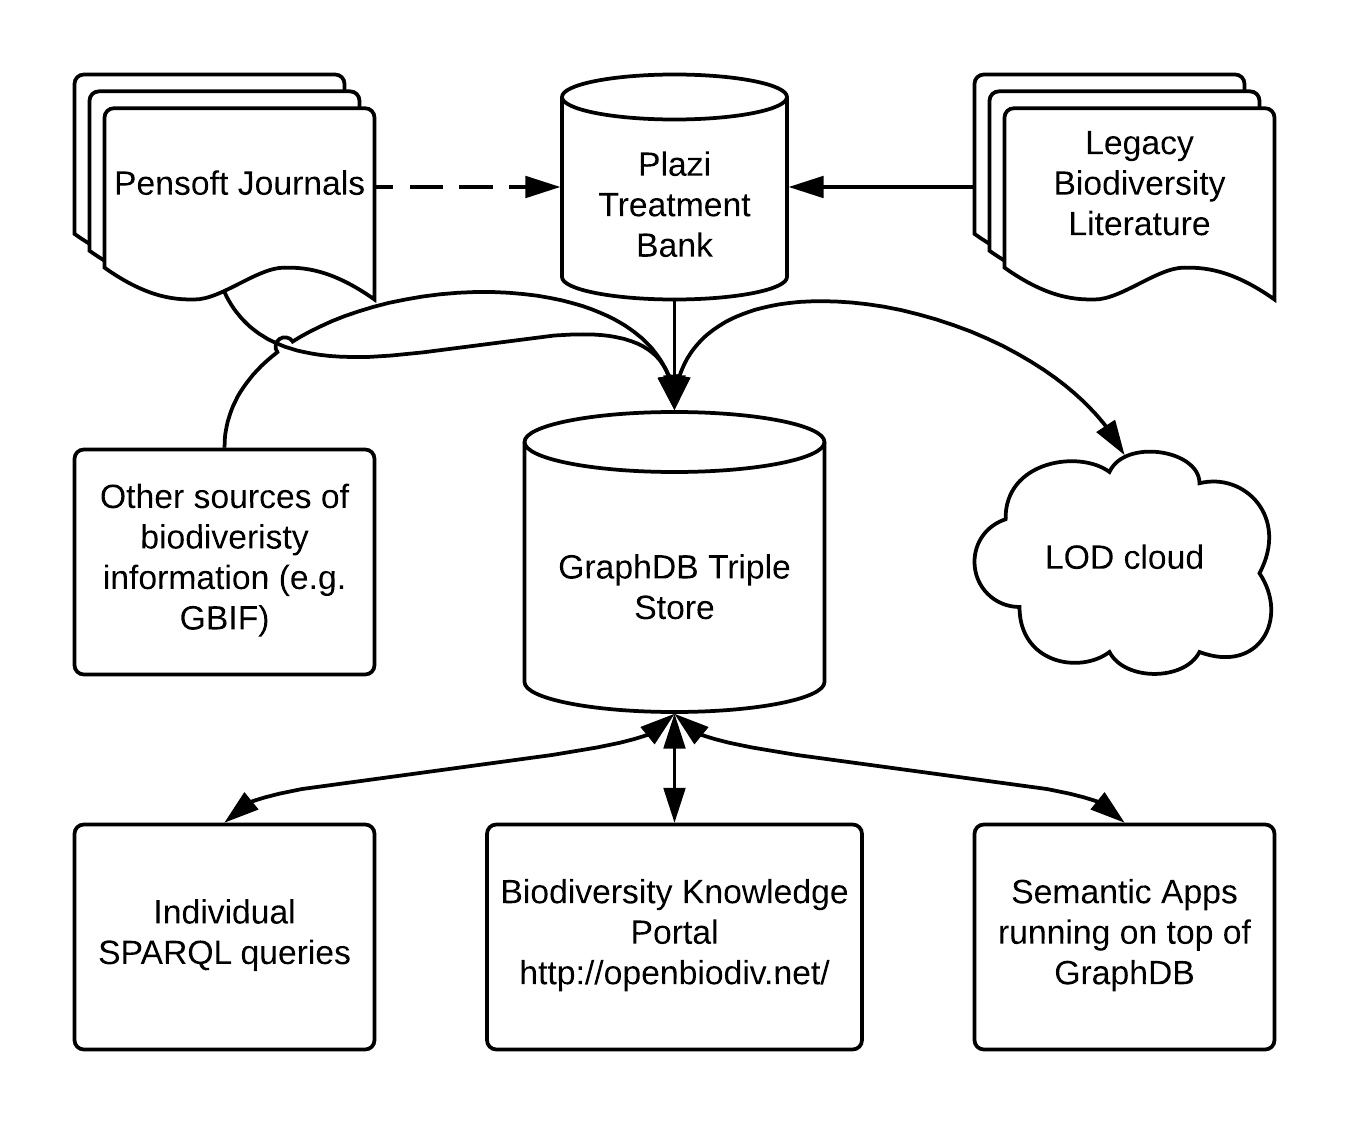
\includegraphics[width=\textwidth]{Figures/openbiodiv-sources-simple}
\decoRule
\caption{Опростен модел на архитектурата на OpenBiodiv от глава~\ref{chapter-openbiodiv} фокусираща върху източниците на информация.}
\label{fig:openbiodiv-sources-simple}
\end{figure}


\subsection{Таксономичен гръбнак на GBIF}

GBIF е най-голямото международно хранилище на данни за наблюдения на организми (occurrence data). GBIF позволява на потребителите да търсят в тяхната система, като използват таксономична йерархия. Например, възможно е да се търсят в базата наблюдения на организми, принадлежащи към определен род: напр. търсене на бръмбар {\textit Harmonia} sec. \cite{gbif_secretariat_gbif_2017-1} на 30 юни 2018 г. върна 575,376 резултата. Това търсене е възможно благодарение на аксономичния гръбнак на GBIF, Nub (\cite{gbif_secretariat_gbif_2017-1}). Nub е база данни, която организира таксономични концепции в йерархия, обхващаща всички имена, събрани от GBIF. Тя е синтетична (алгоритмично генерирана) класификация покриваща всички имена, присъстващи в наборите от данни на GBIF. По този начин гръбнакът GBIF не представлява експертен консенсус за това как таксоните са йерархично подредени според еволюционните критерии в природата.

За да предоставим същите възможности на OpenBiodiv, ние  импортирахме Nub като \cl{openbiodiv:TaxonomicConcept} по OpenBiodiv-O (фиг.~\ref {fig:harmonia-halii-visual}).
\begin{figure}
\centering
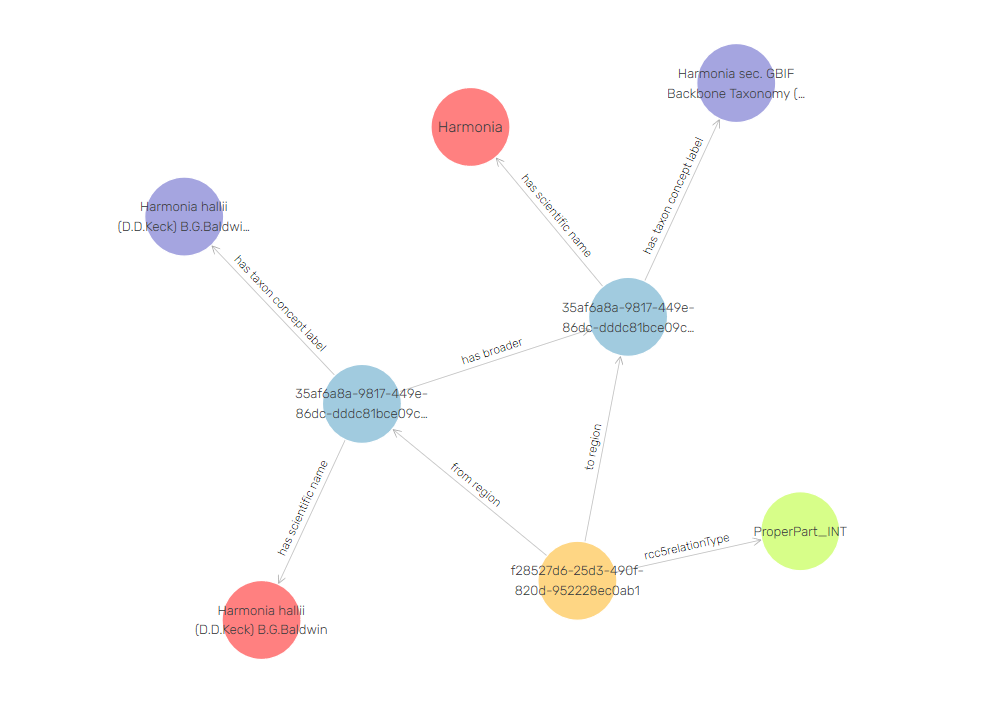
\includegraphics[width=\textwidth]{Figures/harmonia-halii-visgraph}
\decoRule
\caption[Visual graph of \emph{Harmonia halii}]{Илюстрация на представянето на йерархична информаци, импортирана от GBIF като таксономични концепции в OpenBiodiv.}
\label{fig:harmonia-halii-visual}
\end{figure}


\subsection{Пенсфот и Плаци}

Всички валидни статии, от таксономичните списания, публикувани  от Пенсофт и упоменати в Таблица~\ref{rdf-pensoft-journals} бяха конвертирани в RDF и съхранени в графа от знания на биологичното разнообразие. В допълнение, всички валидни таксономични дискусии (treatments) на Плаци бяха конвертирани в RDF и също съхранени в графа. Процедурата по RDF-изиране се повтаря всяка седмица и по този начин семантичната база данни винаги съдържа най-новите статии и таксономични дискусии. RDF-изацията е възможно благодарение на факта, че списанията на Пенсофт публикуват статии в TaxPub XML (\cite{catapano_taxpub:_2010}) докато Плаци публиува дискусиите си в axonX (\cite{penev_xml_2011}) (Fig.~\ref{fig:tnu-vis}). И двете схеми са стандартни и общо-достъпни.

\begin{lstlisting}[language=XML,
caption=Употреба на \emph{P. emarginaticeps} в Taxpub.,
label=listing:tnu, basicstyle=\ttfamily\tiny]
<tp:taxon-name>
  <tp:taxon-name-part taxon-name-part-type="genus" reg="Pristaulacus">
    P.
  </tp:taxon-name-part>
  <tp:taxon-name-part taxon-name-part-type="species" reg="emarginaticeps">
    emarginaticeps
  </tp:taxon-name-part>
  <tp:taxon-name-part taxon-name-part-type="authority">
    Turner 1922
  </tp:taxon-name-part>
</tp:taxon-name> 
\end{lstlisting}

\begin{table}[h!]
\caption{Списания ма Пенсофт, които са превърнати в RDF.}
      \begin{tabular}{ccc}
        \hline
          Journal Name             & Submission Style & Number of Articles\\  \hline
          ZooKeys                 & Word document & 3829\\
          PhytoKeys               & Word document & 537\\
          MycoKeys                & Word document & 127\\
          Biodiversity Data Journal & Web based (ARPHA) & 490\\
          Journal of Orthoptera Research & Word document & 32
      \end{tabular}
      \label{rdf-pensoft-journals}
\end{table}

\begin{table}[h!]
\caption{Типове данни, маркирани в TaxPub and TaxonX и тяхната кореспондеция към RDF типовете, които се използват в OpenBiodiv.}
      \begin{tabular}{cccc}
        \hline
          Datatype             & TaxPub & TaxonX & RDF Type\\  \hline
          Article metadata     & T & T & {\tt fabio:JournalArticle} and related\\
          Keyword group        & T & F & {\tt openbiodiv:KeywordGroup} \\
          Abstract             & T & T & {\tt sro:Abstract}\\
          Title                & T & F & {\tt doco:Title} \\
          Author               & T & T & {\tt foaf:Person} \\
          Introduction section & T & F & {\tt deo:Introduction}\\
          Discussion section   & T & T & {\tt orb:Discussion}\\
          Treatment section    & T & T & {\tt openbiodiv:Treatment}\\
          Nomenclature section & T & T & {\tt openbiodiv:NomenclatureSection}\\
          Materials examined   & T & T & {\tt openbiodiv:MaterialsExamined}\\
          Diagnosis section    & T & T & {\tt openbiodiv:DiagnosisSection} \\
          Distribution section & T & T & {\tt openbiodiv:DistributionSection}\\
          Taxonomic key        & T & T & {\tt openbiodiv:TaxonomicKey}\\
          Figure               & T & T & {\tt doco:Figure}\\
          Taxonomic name usage & T & T & {\tt openbiodiv:TaxonomicNameUsage}
      \end{tabular}
      \label{datatypes-taxpub-taxonx}
\end{table}

\begin{figure}
\centering
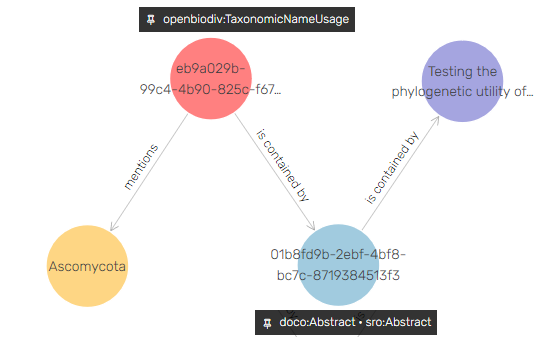
\includegraphics[width=\textwidth]{Figures/tnu-vis}
\decoRule
\caption[Visual graph of a taxonomic name usage]{Употреба на таксономични имена в OpenBiodiv (taxonomic name usage).}
\label{fig:tnu-vis}
\end{figure}

\section{Свързани отворени данни}

Linked Open Data (LOD, \cite{heath_linked_2011}) е идея на Семантичната мрежа (\cite{berners-lee_semantic_2001}) целяща да гарантира полезността на данни публикувани в мрежата, като улеснява тяхното повторно намира и употреба от трети лица. В тази секция разясняваме принципте на свързаните отворени данни и тяхното приложение в OpenBiodiv (\cite{heath_linked_2011}).

\begin{figure}
\centering
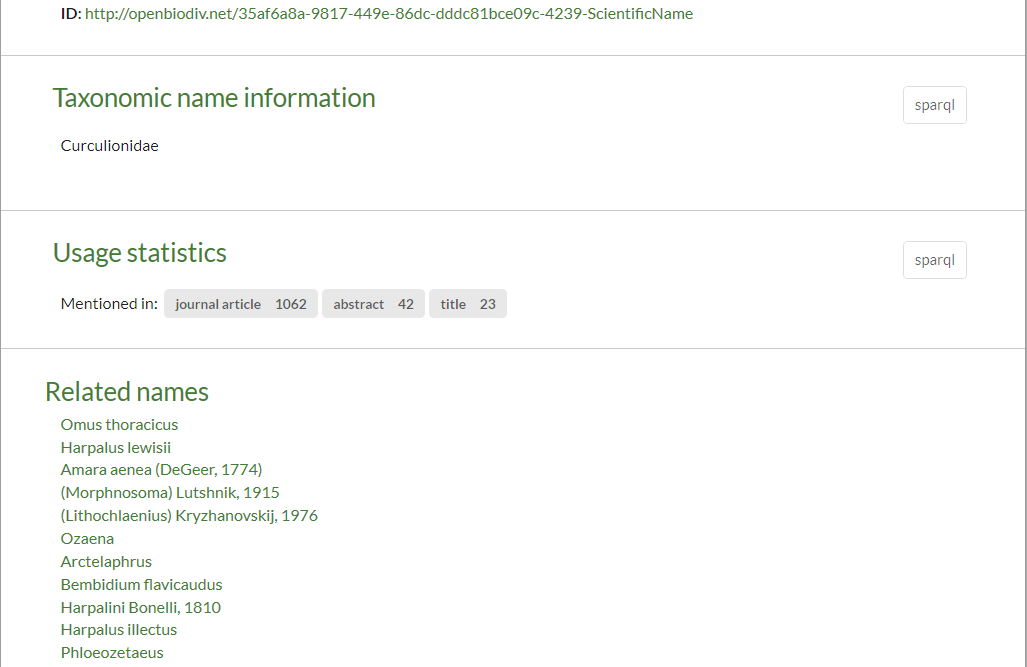
\includegraphics[width=\textwidth]{Figures/portal-name-visualization}
\decoRule
\caption{Визуализация.}
\label{fig:portal-name-visualization}
\end{figure}


\section{Модел на данните}

Подчертаваме, че използваме модела подробно разяснен в глава~\ref{chapter-ontology} и допълнителните онтологии (Fig.~\ref{fig:community-ontologies}).

\begin{figure}
\centering
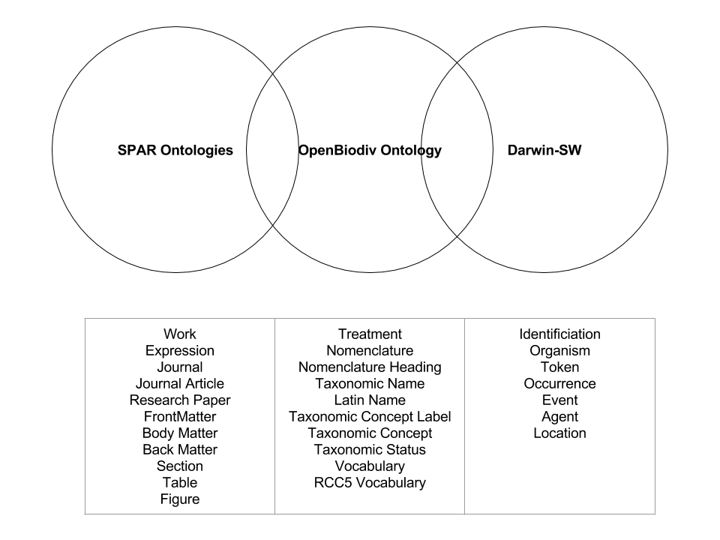
\includegraphics[width=\textwidth]{Figures/community-ontologies}
\decoRule
\caption[Overlap of OpenBiodiv-O with Community Ontologies]{Връзка между OpenBiodiv-O и други публично-достъпни онтологии.}
\label{fig:community-ontologies}
\end{figure}

\section{Примерен SPARQL}

В тази секция илюстрираме, как представеният модел за данни, заедно с инкорпорираната в базата данни информация е достатъчен за да изпълним някои много интересни заявки върху графа за знания.

\subsection{Прости заявки}

В тази подскекция даваме прости заявки. Напр. как да търсим по автори, по научни имена и т.н.

\subsubsection{Заявка върху структурата на статията} 

Тъй като в OpenBiodiv LOD статиите са разбити по тяхните компоненти (вж напр. Таблица~\ref{datatypes-taxpub-taxonx}) и споменаванията на таксони (taxnomic name usages) винаги са свързани със специфична част на статията, може да правим запитвания, използващи тази структура, като напр.:

\subsubsection{Запитване за таксономични концепции}

\subsubsection{Размито търсене с Lucene}

Използваме Lucene connector (\cite{ontotext_graphdb_2018}) на GraphDB, за да допълним точните търсения с размити търсения, където се допускат правописни грашки.

\subsection{Отговаряне на експертни въпроси}

Поради машината си за извод, OpenBiodiv може да функционира като експертна система. В тази подсекция даваме примери за такова запитване:

\subsubsection{Проверка на валидноста на таксономично име}

\subsubsection{Оценка на научната загуба след пожара в Museu Nacional в Бразилия}

Може да запитаме експертната система OpenBiodiv да даде списък с видовете, чиито екземпляри баха загубени в пожара в Рио де Жанейро.

\section{Как създадохме данните?}

В тази секция се разкриват техническите подробности за това, как данните бяха създадени.

\subsection{Получаване на данни}

Дават се адресите в интернет, където данните в суров вид могат да бъдат достъпвани.

\subsection{Инстументи}

Използват се следните инструменти

\begin{enumerate}
\item{Пакет RDF4R}
\item{Пакет ROpenBio}
\item{Пакет TSV4RDF разработен от Пенсофт.}
\item{Базисен код на OpenBiodiv}
\end{enumerate}


\subsection{Трансформация от XML в RDF}

Използваме йерархичната структура на XML, за да решим проблема рекурсивно с помощта на следния Extractor, документиран в Алгоритъм~\ref{algo:extractor}.

% http://tug.ctan.org/macros/latex/contrib/algorithmicx/algorithmicx.pdf
\begin{algorithm}
\caption{Екстрактор}
\begin{algorithmic}[1]
\Procedure {Extractor}{XML Node $X$}
\State $a \leftarrow$ extract atoms of $X$
\Comment Atoms extraction
\State $r \leftarrow$ construct RDF from $a$
\Comment RDF construction
\State $C \leftarrow$ find relevant sub-nodes of $X$
\Comment Recursively applies itself
\State $R \leftarrow$ apply Extractor on each $C_i \in C$
\State \Return $r \bigcup R$
\EndProcedure
\end{algorithmic}
\label{algo:extractor}
\end{algorithm}

\subsubsection{Извличане на атомите}

Текстовите полета в XML ще наричаме атоми. Тяхното извличане се осъществява с помощта на езика XPATH. Тук разясняваме, как става това.

\subsubsection{Генериране на RDF}

След извичане на атомите, те могат да бъдат събрани обратно във формата на RDF.  Пример за генериране на RDF от атомите за даден автор е даден в Listing~\ref{listing:author_rdf}.

\begin{lstlisting}[language=SPARQL,label=listing:author_rdf, caption=RDF за автор на статия., basicstyle=\ttfamily\tiny]
:a a foaf:Person ;
   rdfs:label "Aijaz Ahmad Wachkoo".
   :affiliation "Central Institute of Temperate Horticulture, Srinagar, Jammu & Kashmir, India"@en ;
   foaf:familyName "Wachkoo" ;
   foaf:givenName "Aijaz Ahmad" .
\end{lstlisting}

\begin{lstlisting}[language=SPARQL,
caption=Пример за RDF на метаданните на статия., label=listing:parent-node-rdf, basicstyle=\ttfamily\tiny]
:2b836ad5-db56-4093-9752-33c9f7892de6   rdf:type   fabio:JournalArticle ;
  rdfs:label   "Changes to publication requirements made at the XVIII Internation\
al Botanical Congress in Melbourne - what does e-publication mean for you?" ;
  dc:title   "Changes to publication requirements made at the XVIII International\
 Botanical Congress in Melbourne - what does e-publication mean for you?" ;
 prism:doi   "10.3897/mycokeys.1.1961" ;
 dc:publisher   "Pensoft Publishers" ;
 prism:publicationDate   "2011-9-14"^^xsd:date ;
 dcterms:publisher   openbiodiv:0df76aab-1fcf-4118-8e50-198e830a7bed .
 openbiodiv:151a37ba-a337-4855-8e01-200f5ec0251b   rdf:type   deo:Introduction ;
         po:isContainedBy   openbiodiv:2b836ad5-db56-4093-9752-33c9f7892de6 .
}
\end{lstlisting}

\subsubsection{Стратегия разделяй и владей}

Проблемът за RDF-изиранато на цял XML файл е реализиран посредством разбиването му на малки проблеми, за които решението е тривиално като в горния пример за RDF-изирането на даден автор или на метаданните на дадена статия.

\subsubsection{Дефиниране на трансформацията}

За да работи Extractor, трябва да дефинираме XML схемата. Спецификацията включва какви XML възли търсим и къде се намират. След това рекурсивно се указва за всеки възел кои под-възли търсим и тяхното местоположение на XPATH спрямо техния родителски възел. И накрая, за всеки възел трябва да дадем атомните места и да напишем конструктор. Спецификацията на трансформацията се извършва в R6 калс на R. Определихме две схеми, които споделят същите конструктори: TaxPub\footnote{\url{https://github.com/pensoft/ropenbio/blob/redesign/R/taxpub.R}} и TaxonX \footnote{\url{https://github.com/pensoft/ropenbio/blob/redesign/R/taxonx.R}}.

\subsection{Качване в базата данни и допълнителна обработка}

Извлечените RDF твърдения се изпращат в GraphDB, който се намира на адрес \url{http://graph.openbiodiv.net/}. Освен материазирани твърдения по онтологията, след всеки ъпдейт, изпълняваме следните допълни правила: 

\subsubsection{Ъпдейт на заместващите имена}

Изгражда връзките от тип \cl{РeplacementName} между вмъкнатите имена.
(Listing~\ref{listing:update_replacement_name}).

\lstinputlisting[language=SPARQL,
caption=Ъпдейт на заместващите имена,
label=listing:update_replacement_name, basicstyle=\ttfamily\tiny]{Listings/update-replacement-name.SPARQL.txt}

\subsubsection{Ъпдейт на свързаните имена}

Изгражда връзките между свръзани имена (Listing~\ref{listing:update_related_name}).

\lstinputlisting[language=SPARQL,
caption=Ъпдейт на заместващите имена.,
label=listing:update_related_name, basicstyle=\ttfamily\tiny]{Listings/update-related-name.SPARQL.txt}

\section{Анализ на производителността}

Остановихме, че обемът данни, който обработване в комбинация с пълна OWL логика води до неприемлива производителност. В тази секция разглеждаме този проблем (Фиг.~\ref{fig:statements-report}).

\begin{figure}
\centering
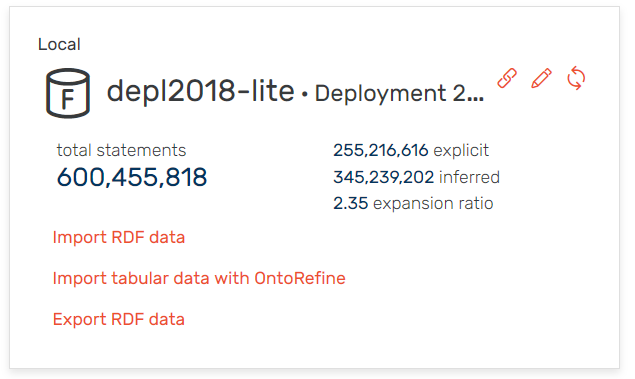
\includegraphics[width=\textwidth]{Figures/active-repository}
\decoRule
\caption[Statements report]{Брой твърдения.}
\label{fig:statements-report}
\end{figure}

\begin{figure}
\centering
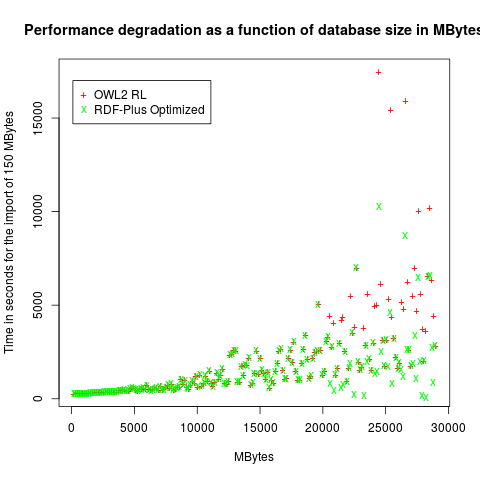
\includegraphics[width=\textwidth]{Figures/performance-degradation-both}
\decoRule
\caption[Performance degradation]{Визуализация на деградацията на производителността.}
\label{fig:performance-degradation}
\end{figure}

